\documentclass[12pt]{article}
\usepackage[margin=1in]{geometry}
\usepackage{graphicx}
\usepackage{booktabs}
\usepackage{amsmath}

\title{The Effect of Paid Search Advertising on Revenue: \\
A Replication of the eBay Natural Experiment}
\author{Aaron Chotzen-Jenner}
\date{\today}

\begin{document}

\maketitle

\section{Introduction}

Firms spend billions of dollars each year on paid search advertising, yet measuring its causal effect on revenue is challenging. The core research question in this paper is: what is the effect of paid search advertising on eBay's revenue? Standard observational comparisons are likely to be biased because advertising intensity is typically correlated with demand conditions. To address this problem, Blake, Nosko, and Tadelis (2014) analyze a natural experiment in which eBay temporarily shut off paid search advertising in selected markets. This paper replicates that empirical strategy using a difference-in-differences (DID) framework to estimate the causal impact of paid search on revenue.

\section{Experimental Setting}

In 2012, Blake et al. (2014) persuaded eBay to stop bidding on Google AdWords in a subset of designated market areas (DMAs). Beginning on May 22, 2012, paid search advertising was turned off in 65 of 210 DMAs, and the treatment lasted for eight weeks. In treatment DMAs, paid search was disabled (search\_stays\_on = 0), while in control DMAs, advertising continued as usual (search\_stays\_on = 1).

Importantly, this was not a fully randomized experiment. The largest DMAs were excluded from the treatment group, meaning that treatment and control markets differ systematically in baseline revenue levels. As a result, a simple comparison of average revenue between treated and untreated markets would be misleading. Instead, the analysis relies on a difference-in-differences design, which compares changes over time between the two groups and accounts for persistent baseline differences.

\section{Data and Figures}

The dataset contains daily revenue observations for 210 DMAs from April through July 2012. Key variables include the date, DMA identifier, an indicator for whether paid search remained active, a post-treatment indicator beginning May 22, and total revenue. This panel structure allows for comparisons across markets and over time surrounding the treatment period.

\begin{figure}[h]
\centering
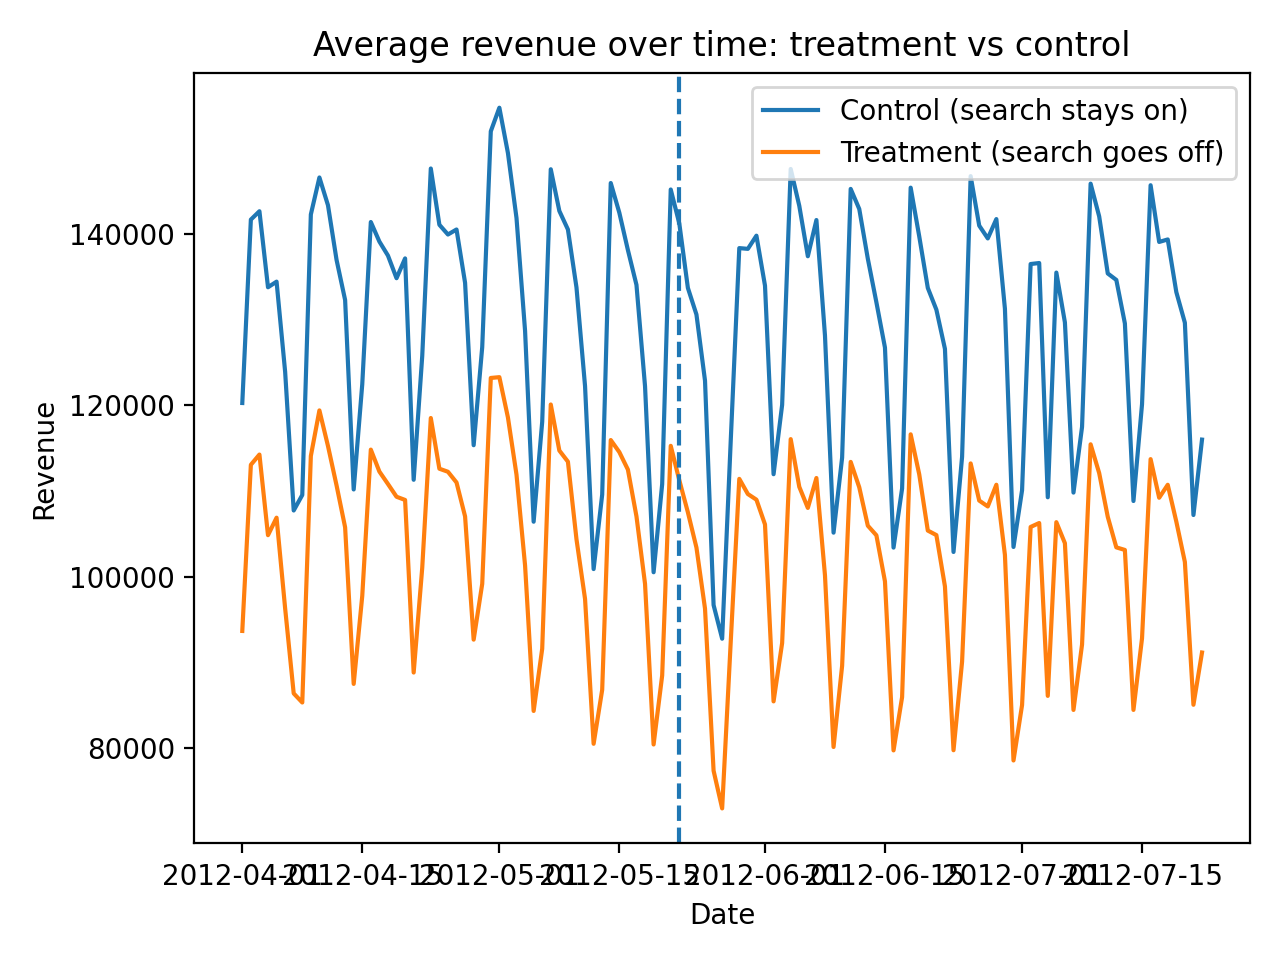
\includegraphics[width=0.85\textwidth]{../output/figures/figure_5_2.png}
\caption{Average revenue for treatment and control DMAs over time.
The dashed line marks May 22, 2012, when SEM was turned off
for the treatment group.}
\label{fig:revenue}
\end{figure}

Figure \ref{fig:revenue} shows average daily revenue for treatment and control DMAs. The control group exhibits higher average revenue throughout the sample, reflecting the exclusion of the largest DMAs from treatment. Both groups display similar weekly oscillation patterns, suggesting comparable demand seasonality. At this scale, there is no obvious divergence in trends after May 22, making it difficult to visually detect a clear treatment effect.

\begin{figure}[h]
\centering
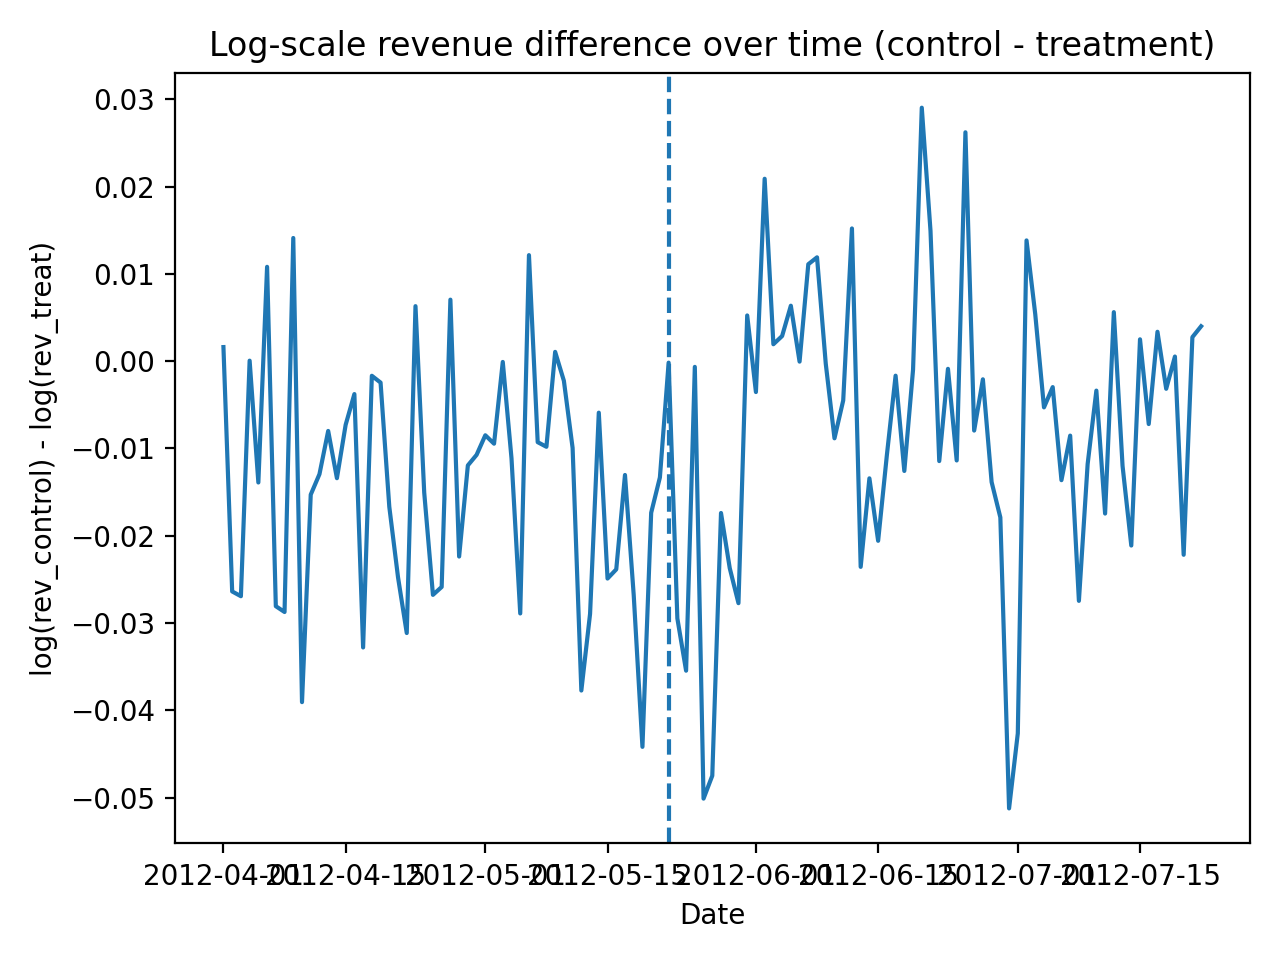
\includegraphics[width=0.85\textwidth]{../output/figures/figure_5_3.png}
\caption{Log-scale average revenue difference between control and treatment
groups over time. The gap appears to increase after May 22.}
\label{fig:logdiff}
\end{figure}

Figure \ref{fig:logdiff} presents the log difference in average revenue between control and treatment groups over time. Prior to May 22, the log revenue gap fluctuates around a relatively stable level, consistent with the parallel trends assumption underlying DID. After the treatment begins, the gap appears to increase slightly, suggesting that treatment markets may have experienced a small decline in revenue relative to control markets. This visual pattern motivates a formal difference-in-differences estimation.

\section{Results}

\input{../output/tables/did_table.tex}

The difference-in-differences estimate of the treatment effect is $\hat{\gamma} = -0.0066$ in log revenue terms. Converting this to percentage terms, $\exp(-0.0066) = 0.9934$, implying that treatment DMAs experienced approximately a 0.66\% decline in revenue after paid search advertising was turned off. 

The 95\% confidence interval for the estimate is [-0.0175, 0.0043], which includes zero. Therefore, the estimated effect is not statistically significant at the 5\% level. Economically, the magnitude of the effect is very small. These findings suggest that turning off paid search advertising had a negligible impact on revenue during the experimental period. One possible interpretation is that for a well-known brand such as eBay, many consumers would have found the site through organic search channels even in the absence of paid ads.

\section{Conclusion}

This replication applies a difference-in-differences framework to estimate the causal effect of paid search advertising on revenue. The results indicate a small and statistically insignificant decline in revenue when advertising was turned off. This finding is consistent with the main conclusion of Blake et al. (2014), who argue that paid search advertising may generate limited incremental value for established brands. 

Several limitations should be noted. The revenue data are scaled and shifted rather than representing true dollar values. The treatment assignment was not fully randomized, and the analysis uses a simple DID specification without additional controls. Nonetheless, the results highlight the importance of experimental or quasi-experimental designs in measuring marketing return on investment.

\begin{thebibliography}{9}

\bibitem{blake2014}
Blake, T., C. Nosko, and S. Tadelis (2014).
``Consumer Heterogeneity and Paid Search Effectiveness: A Large-Scale Field Experiment.''
\textit{Econometrica}, 83(1): 155--174.

\bibitem{taddy2019}
Taddy, M. (2019).
\textit{Business Data Science}. McGraw-Hill, Chapter 5.

\end{thebibliography}

\end{document}
